\RequirePackage{luatex85}
\documentclass[border=1pt]{standalone}
\usepackage{tikz}
\usetikzlibrary{shapes.geometric, arrows}

\tikzstyle{normal} = [rectangle, rounded corners, minimum width=3cm, text width=3cm, minimum height=1cm,text centered, draw=black, fill=green!60]
\tikzstyle{smalln} = [rectangle, rounded corners, minimum width=1.5cm, text width=2cm, minimum height=1cm, font=\small, text centered, draw=black, fill=green!60]
\tikzstyle{new} = [rectangle, minimum width=3cm, text width=3cm, minimum height=1cm, text centered, draw=black, fill=yellow!60]
\tikzstyle{smallnew} = [rectangle, rounded corners, minimum width=1.5cm, text width=3cm, minimum height=1cm, font=\small, text centered, draw=black, fill=yellow!60]
\tikzstyle{decision} = [diamond, minimum width=3cm, minimum height=1cm, text centered, draw=black, fill=green!30]
\tikzstyle{cloud} = [ellipse, minimum width=3cm, text width=3cm, minimum height=1cm, text centered, draw=black, fill=orange!30]
\tikzstyle{arrow} = [thick,->,>=stealth]



\begin{document}
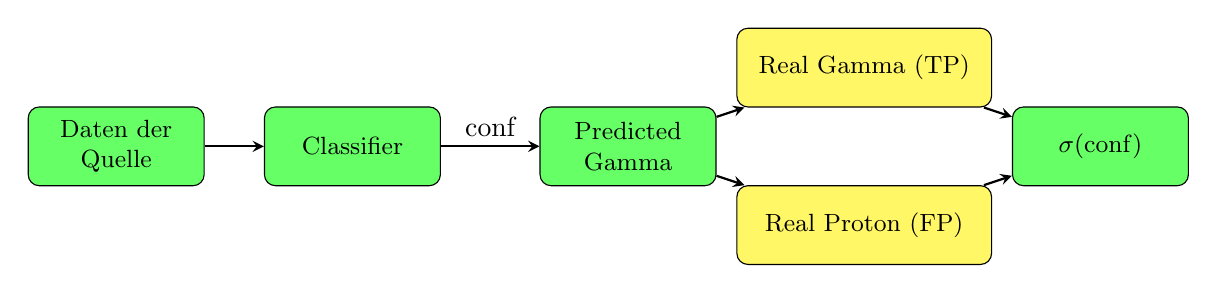
\begin{tikzpicture}[node distance=1cm]
  \node (RAW) [smalln] {Daten der Quelle};
  \node (CLAS) [smalln, right of=RAW, xshift=2cm] {Classifier};
  \node (PRED) [smalln, right of=CLAS, xshift=2.5cm] {Predicted Gamma};
  \node (RGAM) [smallnew, right of=PRED, xshift=2cm, yshift=1cm] {Real Gamma (TP)};
  \node (RPRO) [smallnew, right of=PRED, xshift=2cm, yshift=-1cm] {Real Proton (FP)};
  \node (SIGM) [smalln, right of=RGAM, xshift=2cm, yshift=-1cm] {$\sigma$(conf)};

  \draw [arrow] (RAW) -- (CLAS);
  \draw [arrow] (CLAS) -- node[anchor=south] {conf} (PRED);
  \draw [arrow] (PRED) -- (RGAM);
  \draw [arrow] (PRED) -- (RPRO);
  \draw [arrow] (RGAM) -- (SIGM);
  \draw [arrow] (RPRO) -- (SIGM);
\end{tikzpicture}
\end{document}
